\documentclass[a4paper,11pt]{report}

\usepackage{graphics}
\usepackage{graphicx}
\usepackage{booktabs}
\usepackage{array}

\def\complement#1{#1'}

\usepackage{tikz, ifthen}
\usetikzlibrary{arrows,shapes,backgrounds,patterns,decorations.pathreplacing,decorations.pathmorphing}

\def\makedieempty#1#2{
  \begin{scope}[#1]
    \pgfsetcornersarced{\pgfpoint{#2}{#2}}
    \draw (-0.5cm, -0.5cm) rectangle (0.5cm, 0.5cm);
  \end{scope}
}

\def\makedieone#1#2{
  \begin{scope}[#1]
    \pgfsetcornersarced{\pgfpoint{#2}{#2}}
    \draw (-0.5cm, -0.5cm) rectangle (0.5cm, 0.5cm);
    \fill[black] (0, 0) circle (0.125);
  \end{scope}
}

\def\makedietwo#1#2{
  \begin{scope}[#1]
    \pgfsetcornersarced{\pgfpoint{#2}{#2}}
    \draw (-0.5cm, -0.5cm) rectangle (0.5cm, 0.5cm);
    \fill[black] (-0.3, -0.3) circle (0.125);
    \fill[black] (0.3, 0.3) circle (0.125);
  \end{scope}
}

\def\makediethree#1#2{
  \begin{scope}[#1]
    \pgfsetcornersarced{\pgfpoint{#2}{#2}}
    \draw (-0.5cm, -0.5cm) rectangle (0.5cm, 0.5cm);
    \fill[black] (-0.3, -0.3) circle (0.125);
    \fill[black] (0, 0) circle (0.125);
    \fill[black] (0.3, 0.3) circle (0.125);
  \end{scope}
}

\def\makediefour#1#2{
  \begin{scope}[#1]
    \pgfsetcornersarced{\pgfpoint{#2}{#2}}
    \draw (-0.5cm, -0.5cm) rectangle (0.5cm, 0.5cm);
    \fill[black] (-0.3, -0.3) circle (0.125);
    \fill[black] (0.3, -0.3) circle (0.125);
    \fill[black] (0.3, 0.3) circle (0.125);
    \fill[black] (-0.3, 0.3) circle (0.125);
  \end{scope}
}

\def\makediefive#1#2{
  \begin{scope}[#1]
    \pgfsetcornersarced{\pgfpoint{#2}{#2}}
    \draw (-0.5cm, -0.5cm) rectangle (0.5cm, 0.5cm);
    \fill[black] (0, 0) circle (0.125);
    \fill[black] (-0.3, -0.3) circle (0.125);
    \fill[black] (0.3, -0.3) circle (0.125);
    \fill[black] (0.3, 0.3) circle (0.125);
    \fill[black] (-0.3, 0.3) circle (0.125);
  \end{scope}
}

\def\makediesix#1#2{
  \begin{scope}[#1]
    \pgfsetcornersarced{\pgfpoint{#2}{#2}}
    \draw (-0.5cm, -0.5cm) rectangle (0.5cm, 0.5cm);
    \fill[black] (-0.3, -0.3) circle (0.125);
    \fill[black] (-0.3,  0.0) circle (0.125);
    \fill[black] (-0.3,  0.3) circle (0.125);
    \fill[black] ( 0.3, -0.3) circle (0.125);
    \fill[black] ( 0.3,  0.0) circle (0.125);
    \fill[black] ( 0.3,  0.3) circle (0.125);
  \end{scope}
}

\def\makediegeneral#1#2#3{
  \ifthenelse{#1=1}{\makedieone{#2}{#3}}{
    \ifthenelse{#1=2}{\makedietwo{#2}{#3}}{
      \ifthenelse{#1=3}{\makediethree{#2}{#3}}{
        \ifthenelse{#1=4}{\makediefour{#2}{#3}}{
          \ifthenelse{#1=5}{\makediefive{#2}{#3}}{
            \ifthenelse{#1=6}{\makediesix{#2}{#3}}{
              \makedieempty{#2}{#3}}}}}}}
}

\def\makedie#1#2{
  \makediegeneral{#1}{#2}{0.175cm}
}

\def\makediesmall#1#2{
  \makediegeneral{#1}{#2}{0.0875cm}
}


\begin{document}
\chapter{Probability}

\section{Introduction}

We use probability to describe uncertain events. When you accidentally
drop a slice of bread, you don't know if it's going to fall with the
buttered side facing upwards or downwards.

[IMPLICIT? There are different kinds of uncertainties: lack of
information, model misalignment]

Probability and uncertainty in everyday life: the chance that it's
going to rain tomorrow (e.g. 20\%); the chances that Bafana Bafana
will win a soccer match (50--50, or ``1 in 2'').

We will see in this chapter that all of these uncertainties can be
described using the rules of probability theory and that we can make
conclusions about uncertain events and processes.

\section{Definitions}

We'll use the following three examples of uncertain processes to help
you understand the meanings of the different words used in probablity
theory. We use the term {\em experiment} to refer to an uncertain process.

\paragraph{Experiment 1} A coin is tossed and it lands with either heads
(H) or tails (T) facing upwards.

FIGURE: coin

\paragraph{Experiment 2} Two dice are rolled and the total number of dots
added up.

\begin{center}
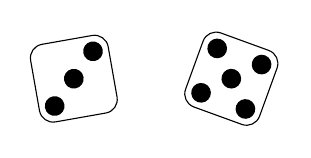
\begin{tikzpicture}
  \makedie{3}{shift={(-1,0)},rotate=10}
  \makedie{5}{shift={(1,0)},rotate=-20}
\end{tikzpicture}
\end{center}

\paragraph{Experiment 3} Two teams play in a soccer match and we are
interested in the final score.

FIGURE: soccer score board

Each of the figures for the experiments show one possible outcome.

\paragraph{Definition} The {\em outcome} of an experiment is the single
result of that experiment.

Even though we are usually interested in the outcome of an experiment,
we also need to know what the other outcomes could have been.

\paragraph{Definition} The {\em sample space} of an experiment is the
set of all possible outcomes of that experiment. The sample space is
denoted with the symbol \(S\) and the size of the sample space (the
total number of possible outcomes) is denoted with \(n(S)\).

\paragraph{Experiment 1} Since a coin can land in one of only two ways
(we will ignore the possibility that the coin lands on its edge), the
sample space is the set \(S=\{H, T\}\). The size of the sample space
is \(n(S)=2\).

FIGURE: sample space box around H and T

\paragraph{Experiment 2} Each of the dice can land on a number from 1
to 6. In this experiment the sample space of all possible outcomes is
every possible combination of the 6 numbers on the first die with the
6 numbers on the second die. This gives a total of \(n(S) = 6 \times 6 = 36\)
possible outcomes. The figure below shows all of the possibilities in
the sample space.

\begin{center}
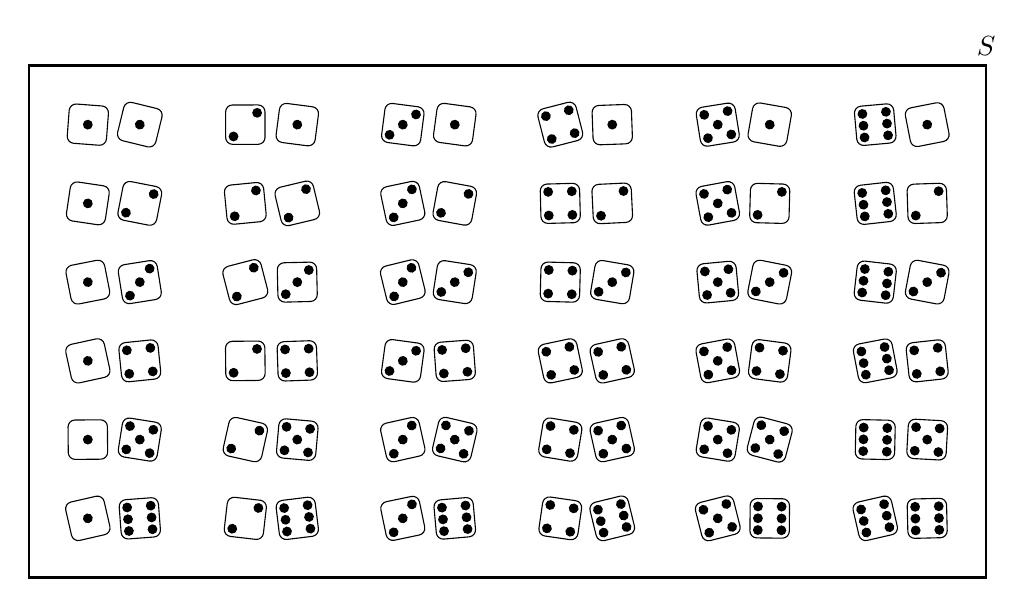
\begin{tikzpicture}
  \begin{scope}[scale=0.5]
  \foreach \x in {1, ..., 6} {
    \foreach \y in {1, ..., 6} {
      \pgfmathparse{15*rand} \let\rot\pgfmathresult
      \makediesmall{\x}{shift={(4cm*\x-0.66cm,-2cm*\y)},rotate=\rot}
      \pgfmathparse{15*rand} \let\rot\pgfmathresult
      \makediesmall{\y}{shift={(4cm*\x+0.66cm,-2cm*\y)},rotate=\rot}
    }
  }
  \draw[thick] (2.5cm-0.66cm, -0.5cm) rectangle (25.5cm+0.66cm, -13.5cm);
  \draw (25.5cm+0.66cm, -0.5cm) node[anchor=south] {$S$};
  \end{scope}
\end{tikzpicture}
\end{center}

\paragraph{Experiment 3} Each team can get an integer score from 0
upwards. Usually we don't expect a score to go much higher than 5
goals, but there is no reason why this cannot happen. So the sample
space of this experiment consists of all possible combinations of two
non-negative integers. The figure below shows all of the
possibilities. Since we do not limit the score of a team, this sample
space is infinitely large.

FIGURE: open-ended sample space box showing all possible pairs of integers

When looking at the set of possible outcomes of an experiment, we are
usually interested in some subset of them.

\paragraph{Definition} An {\em event} is a specific set of outcomes of
an experiment that you are interested in. An event is denoted with the
letter \(E\) and the number of outcomes in the event with \(n(E)\).

\paragraph{Experiment 1} We would like the coin to land heads up. Here
the event contains a single outcome \(E=\{\textrm{H}\}\), \(n(E)=1\).

\paragraph{Experiment 2} Let's say that we are interested in the sum
of the dice being 8. In this case the event set is
\(E=\{(2,6),(3,5),(4,4),(5,3),(6,2)\}\) with \(n(E)=5\). We can also
represent this visually by drawing a line around the outcomes in which
we are interested.

FIGURE: sample space with closed curve around event set

\paragraph{Experiment 3} We would like to know whether the first team
will win. For this to happen the first score must be greater than the
second. \(E=\{(1,0),(2,0),(2,1),(3,0),(3,1),(3,2),\ldots\}\).

FIGURE: sample space with open curve around event set

\section{Theoretical probability}
A {\em probability} is a number that describes how likely it is that
an event will occur. We write probabilities as real numbers between 0
and 1.
\begin{itemize}
\item 0 means that an event will never occur.
\item 1 means that an event will always occur.
\item 0.5 means that an event will occur half the time.
\item etc.
\end{itemize}
People sometimes write probabilities in other forms: as percentages,
as fractions, as odds.

When all of the possible outcomes of an experiment have an equal
chance of occurring, we can compute the exact theoretical probability
of an event occurring. The probability of an event is the ratio
between the number of outcomes in the event to the number of possible
outcomes.
\[P(E) = \frac{n(E)}{n(S)}\]

\paragraph{Experiment 1} The number of outcomes in the event set is
\(n(E)=1\). The size of the sample space is \(n(S)=2\). Since each of
the outcomes (heads or tails) is equally likely, we can compute the
theoretical probability of the coin landing heads up as
\[P(E) = \frac{n(E)}{n(S)} = \frac{1}{2} = 0.5\]

\paragraph{Experiment 2} The number of outcomes in the event set is
\(n(E)=5\). The size of the sample space is \(n(S)=36\). Since each of
the outcomes (each number combination of two dice) is equally likely,
we can compute the theoretical probability of the sum of the dice being 8 as
\[P(E) = \frac{n(E)}{n(S)} = \frac{5}{36} = 0.13\dot{8}\]

\paragraph{Experiment 3} This experiment is different from the
previous experiments in an important way, namely that all possible
outcomes (all final scores) are not equally likely. For example, we
know that a score of 1--1 is quite common, while a score of 11--15 is
very, very rare. (Interesting fact: the record for most goals score by
both teams in the FIFA World Cup is 12 in 1954 in the match between
Austria and Switzerland where the final score was 7--5.)  Because all
outcomes are not equally likely, we cannot use the ratio between
\(n(E)\) and \(n(S)\) to compute the theoretical probability of a team
winning. Outside of the scope of this chapter.

\section{Relative Frequency}
The relative frequency of an event is defined as the number of times
that the event occurs during experimental trials, divided by the total
number of trials conducted. The relative frequency is not a
theoretical quantity, but an experimental one. We have to repeat an
experiment a number of times and count how many times the outcome of
the experiment is in the event set.

\paragraph{Experiment 1} We toss the coin 40 times and observe the
following outcomes after each trial. In the table above, $t$ counts
the number of trials that have been performed, $p$ counts the number
of positive outcomes (when we observe heads) and $f$ shows the
relative frequency after the number of trials that have already been
completed. Since the relative frequency is defined as the ratio
between the number positive trials and the total number of trials
\[f=\frac{p}{t}\]

\begin{tabular}{cccc|cccc|cccc|cccc}
  \toprule
  $t$ && $p$ & $f$  & $t$ && $p$ & $f$  & $t$ && $p$ & $f$  & $t$ && $p$ & $f$\\
  \midrule
  1 & H & 1 & 1.00 & 11 & H & 6 & 0.55 & 21 & H &  9 & 0.43 & 31 & T & 13 & 0.42\\
  2 & T & 1 & 0.50 & 12 & T & 6 & 0.50 & 22 & H & 10 & 0.45 & 32 & H & 14 & 0.44\\
  3 & T & 1 & 0.33 & 13 & T & 6 & 0.46 & 23 & H & 11 & 0.48 & 33 & H & 15 & 0.45\\
  4 & T & 1 & 0.25 & 14 & H & 7 & 0.50 & 24 & T & 11 & 0.46 & 34 & H & 16 & 0.47\\
  5 & H & 2 & 0.40 & 15 & T & 7 & 0.47 & 25 & H & 12 & 0.48 & 35 & H & 17 & 0.49\\
  6 & T & 2 & 0.33 & 16 & T & 7 & 0.44 & 26 & T & 12 & 0.46 & 36 & H & 18 & 0.50\\
  7 & H & 3 & 0.43 & 17 & T & 7 & 0.41 & 27 & H & 13 & 0.48 & 37 & T & 18 & 0.49\\
  8 & H & 4 & 0.50 & 18 & H & 8 & 0.44 & 28 & T & 13 & 0.46 & 38 & H & 19 & 0.50\\
  9 & H & 5 & 0.56 & 19 & T & 8 & 0.42 & 29 & T & 13 & 0.45 & 39 & H & 20 & 0.51\\
  10 & T & 5 & 0.50 & 20 & T & 8 & 0.40 & 30 & T & 13 & 0.43 & 40 & H & 21 & 0.53\\
  \bottomrule
\end{tabular}

From the last row of this table we can now easily read the relative
frequency after 40 trials, namely $21/40 = 0.53$. The relative
frequency is close to the theoretical probability of 0.5. In general,
the relative frequency of an event gets closer to the theoretical
probability of the event as we perform more trials.

We can observe how the relative frequency approaches the theoretical
probability in the plot below. The plot was generated from the table
of numbers above and shows the relative frequency, $f$, as a function
of the number of trials, $t$. In the beginning the relative frequency
fluctuates a lot around the theoretical probability at 0.5 (shown with
a dashed line). As the number of trials increases, the relative
frequency fluctuates less and gets closer to the theoretical
probability.

\begin{center}
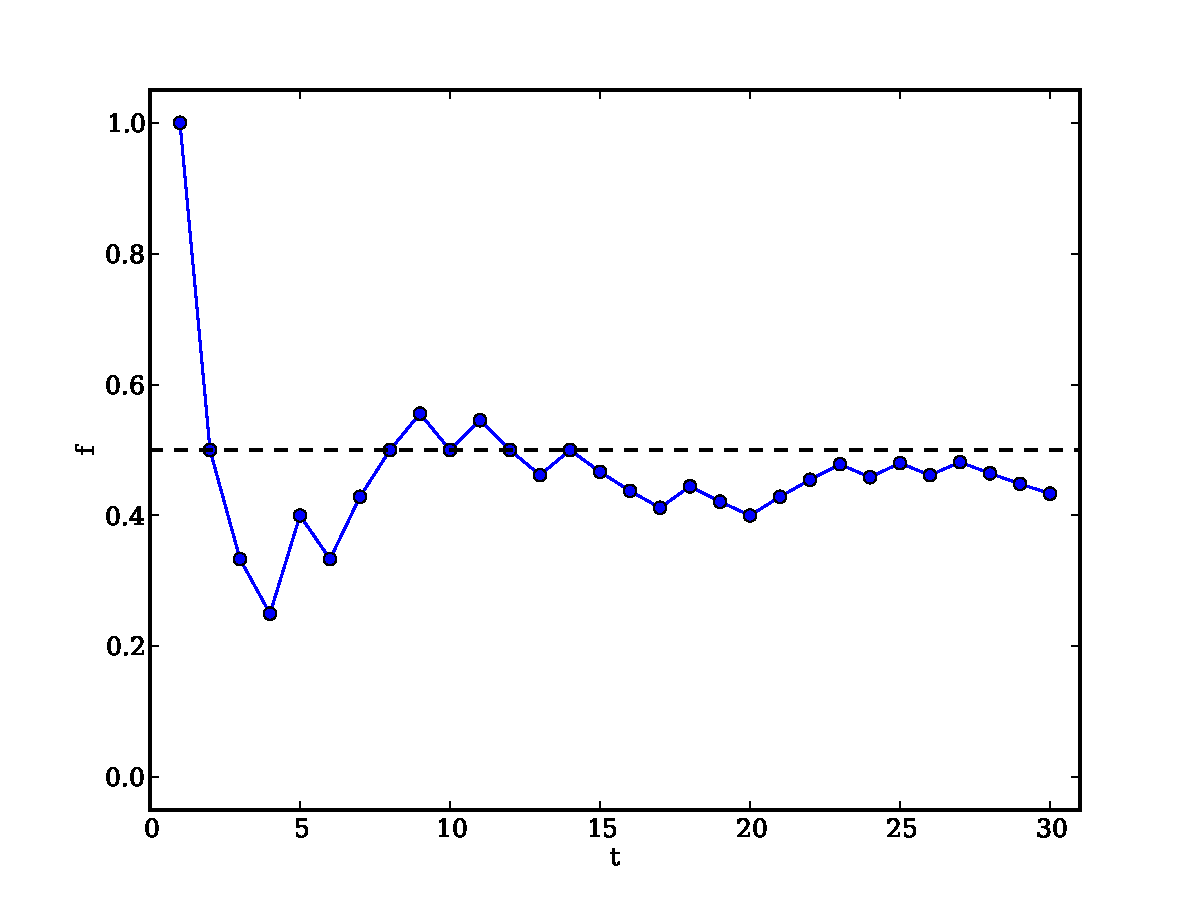
\includegraphics[width=0.75\textwidth]{coin_toss_trials.pdf}
\end{center}

\paragraph{Experiment 2} We roll the two dice 100 times and observe
whether the sum of the dice equals 8. It turns out that our event
occurs 15 times during the experiment. From this we can calculate the
relative frequency as
\[\frac{15}{100}=0.15\]
This is close to the theoretical probability, which we compute earlier
as $0.13\dot{8}$.

\paragraph{Experiment 3} While watching 10 soccer games where Team 1
plays against Team 2, we record the following final scores.
\begin{center}
\begin{tabular}{lcccccccccc}
  \toprule
  Trial  & 1 & 2 & 3 & 4 & 5 & 6 & 7 & 8 & 9 & 10 \\
  \midrule
  Team 1 & 2 & 0 & 1 & 1 & 1 & 1 & 1 & 0 & 5 & 3 \\
  Team 2 & 0 & 2 & 2 & 2 & 2 & 1 & 1 & 0 & 0 & 0 \\
  \bottomrule
\end{tabular}
\end{center}
We are interested in the event where Team 1 wins. From the table above
we see that this happens 3 times out of 10. This means that the
relative frequency of the event is
\[\frac{3}{10} = 0.3\]

It is important to understand the difference between the theoretical
probability of an event and the observed relative frequency of an
experiment. The theoretical probability is a number that we can
compute if we have enough information about the experiment. If the
each possible outcome in the sample space is equally likely, we can
count the number of outcomes in the event set and the number of
outcomes in the sample space to compute the theoretical probability.

The relative frequency depends on the sequence of outcomes that we
observe while doing a statistical experiment. The relative frequency
can be different every time we redo the experiment. The more trials we
run during an experiment, the closer the observed relative frequency
of an event will get to the theoretical probability of the event.

In some cases, like our Experiment 3, it is difficult or impossible to
compute the theoretical probability of an event. Since we do not know
exactly how likely it is that one soccer team will score goals against
another, we can never compute the theoretical probability of events in
soccer. In such cases we can still use the relative frequency to
estimate the theoretical probability by running experiments and
counting the number of positive outcomes.

\section{Venn diagrams}
A Venn diagram is a tool for showing the relationships between
sets. It is helpful for thinking about probability since we deal with
different sets --- so far we have seen the sample space, $S$, and an
event set, $E$.

Consider two possible events, $A$ and $B$, in a sample space $S$. Below
are the possible ways in which the event sets can overlap, represented
using Venn diagrams. In each Venn diagram a set is represented by a
closed curve: a rectangle for $S$ and circles for each of $A$ and $B$.
The space inside a region represents all of the elements included in a
set, while the space outside a region represents the elements excluded
from a set.

FIGURE VENN 1

\paragraph{Example} We can represent the sample space of two rolled dice
and the events
\begin{itemize}
\item $A:$ The sum of the dice equals 8
\item $B:$ At least one of the dice shows
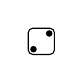
\begin{tikzpicture}
  \begin{scope}[scale=0.333]
    \makediegeneral{2}{}{0.175cm*0.333}
  \end{scope}
\end{tikzpicture}
\end{itemize}
as a Venn diagram.

FIGURE VENN DICE: sum=8 and at least one 2

We will see in the following section how Venn diagrams can be used to
represent and prove some theorems about probabilities.

\section{Union and intersection}
The union of two sets, $A$ and $B$, is a new set that contains all of
the elements that are in $A$, or in $B$, or in both of them. The union
is written as $A \cup B$.

The intersection of $A$ and $B$ is a new set that contains all of the
elements that are in both $A$ and $B$. The intersection is written as
$A \cap B$.

The figure below shows the union and intersection of two event sets in
a sample space, using Venn diagrams.

\def\samplespace{(0,0) rectangle (1,1)}
\def\labelsamplespace{\draw (1,1) node[anchor=south] {$S$}}

\def\circlepartiala{(0.25,0.5) circle (0.2)}
\def\labelpartiala{\draw (0.25,0.7) node[anchor=south] {$A$}}
\def\circlepartialb{(0.6,0.4) circle (0.3)}
\def\labelpartialb{\draw (0.6,0.7) node[anchor=south] {$B$}}

\def\circleseparatea{(0.2,0.3) circle (0.1)}
\def\labelseparatea{\draw (0.23,0.25) node[anchor=north west] {$A$}}
\def\circleseparateb{(0.5,0.6) circle (0.2)}
\def\labelseparateb{\draw (0.5,0.8) node[anchor=south] {$B$}}

\def\circlefulla{(0.5,0.5) circle (0.35)}
\def\labelfulla{\draw (0.75,0.75) node[anchor=south west] {$A$}}
\def\circlefullb{(0.5,0.6) circle (0.15)}
\def\labelfullb{\draw (0.5,0.45) node[anchor=north] {$B$}}


Notes
\begin{itemize}
\item In the middle column the intersection, $A \cap B$, is empty
  since the two sets do not overlap.
\item In the final column the union, $A \cup B$, is equal to $A$ since
  $B$ is fully contained in $A$.
\item In the final column the intersection, $A \cap B$, is equal to
  $B$ since $B$ is fully contained in $A$.
\end{itemize}

\section{Probability identities}
The first identity states that the probability of observing an outcome
from the whole sample space is 1.
\[P(S)=1\]
In other words, every outcome from an experiment must be in the sample
space, $S$. This follows directly from the definition of {\em sample
  space}, namely that it is the set of all possible outcomes.

The second identity relates the union and intersection of two sets:
\[P(A \cup B) = P(A) + P(B) - P(A \cap B)\]

Refer back to VENN 2 from which you can see this identity by adding
the area of circle A to circle B and subtracting intersection area =>
this gives exactly the union area. The common steps are that adding
\(P(A)\) and \(P(B)\) counts \(P(A \cap B)\) twice, so by subtracting
\(P(A \cap B)\) once we get exactly \(P(A \cup B)\).

Work through it visually work one of the columns

\begin{center}
\begin{tabular}{m{0.5cm}m{1.5cm}m{0.5cm}m{1.5cm}m{0.5cm}m{1.5cm}}
   & $P(A)$ & $+$ & $P(B)$ & $-$ & $P(A \cap B)$ \\
 = & \begin{tikzpicture}
   \begin{scope}[scale=1]
     \draw \samplespace;
     \draw[fill=lightgray] \circlepartiala;
   \end{scope}
\end{tikzpicture} & $+$ & \begin{tikzpicture}
   \begin{scope}[scale=1]
     \draw \samplespace;
     \draw[fill=lightgray] \circlepartialb;
   \end{scope}
\end{tikzpicture} & $-$ & \begin{tikzpicture}
   \begin{scope}[scale=1]
     \draw \samplespace;
     \draw[fill=lightgray] (0.31369, 0.31041) arc (197.38:130.73:0.3cm) arc (39.54:-71.43:0.2cm);
   \end{scope}
\end{tikzpicture} \\
 = & \begin{tikzpicture}
   \begin{scope}[scale=1]
     \draw \samplespace;
     \draw[fill=lightgray] \circlepartiala;
   \end{scope}
\end{tikzpicture} & $+$ & \begin{tikzpicture}
   \begin{scope}[scale=1]
     \draw \samplespace;
     \draw[fill=lightgray] (0.31369, 0.31041) arc (-162.62:130.73:0.3cm) arc (39.54:-71.43:0.2cm);
   \end{scope}
\end{tikzpicture} \\
 = & \begin{tikzpicture}
      \begin{scope}[scale=1]
        \draw \samplespace;
        \draw[fill=lightgray] (0.31369, 0.31041) arc (-162.62:130.73:0.3cm) arc (39.54:288.57:0.2cm);
      \end{scope}
\end{tikzpicture} \\
 = & $P(A \cup B)$ \\
\end{tabular}
\end{center}

\paragraph{Experiment 2} We can related the union, intersection for
this experiment: What is the probability of the sum of two
rolled dice equalling 8 or at least one of the dice showing a 2.
\begin{eqnarray*}
  P(A) &=& 5/36 \\
  P(B) &=& 11/36 \\
  P(A \cap B) &=& 2/36 \\
  P(A \cup B) &=& 14/35
\end{eqnarray*}

\section{Mutually exclusive events}
Two events are called {\em mutually exclusive} if they cannot occur at
the same time. Whenever an outcome of an experiment is in the first
event it can not also be in the second event.

Another way of saying this is that the two event sets, $A$ and $B$,
cannot have any elements in common, or $P(A \cap B) = \emptyset$
(where $\emptyset$ denotes the empty set).

VENN2 middle column shows venn diagrams for mutually exclusive
events. You can see that the intersection has no elements. You can
also see that the union $P(A \cup B) = P(A) + P(B)$. This relationship
is true for mutually exclusive events only.

\paragraph{Example} When rolling 2 dice, show that the following two
events are mutually exclusive:
\begin{itemize}
\item $A:$ The sum of the dice equals 8
\item $B:$ At least one of the dice shows

\begin{tikzpicture}
  \begin{scope}[scale=0.333]
    \makediegeneral{1}{}{0.175cm*0.333}
  \end{scope}
\end{tikzpicture}
\end{itemize}
Draw the sample space and the two sets. Notice that there are no
elements in common. Therefore the event sets are mutually exclusive.

\section{Complementary events}

\paragraph{Definition} The {\em complement} of a set, $A$, is a
different set that contains all of the elements that are not in
$A$. We write the complement of $A$ as $\complement{A}$, or sometimes
as ``$\textrm{not}(A)$''.

For an experiment with sample space $S$ and an event $A$ we can derive
some identities for complementary events.
\begin{itemize}
\item Since every element in $A$ is not in $\complement{A}$, we know
  that complementary events are mutually exclusive.
  \[A \cap \complement{A} = \emptyset\]
\item Since every element in the sample space is either in $A$ or in
  $\complement{A}$, the union of complementary events covers the
  sample space.
  \[A \cup \complement{A} = S\]
\item From the previous two identities, we also know that the
  probabilities of complementary events sum to 1.
  \[P(A) + P(\complement{A}) = P(A \cup \complement{A}) = P(S) = 1\]
\end{itemize}

EXERCISES (only at end of chapter?)

\end{document}
